\documentclass{article}
\usepackage{graphicx}
\usepackage[utf8]{inputenc}
\usepackage[T1]{fontenc}
\usepackage{amsmath}
\usepackage{algorithm,algorithmic}
\usepackage{booktabs}

\title{Raport z wykonania zadania}
\author{Maciej Ciepiela}
\date{\today}

\begin{document}

\maketitle

\vspace{2cm}
\section{Część A}
\subsection{Opis rozwiązania}

Do generowania zróżnicowanych grafów stworzyłem klase RandomGraph,
która automatycznie inicjalizuje się na podaną liczbę wierzchołków.
Po czym losuje liczbę krawędzi z przedziału od $n-2$ do $n^2$, gdzie $n$ to liczba wierzchołków.
Następnie losuje wierzchołki, które połączy krawędź. 
Liczba krawędzi może wydawać się duża, ale jest celowa ze względu na potrzeby zadania i fakt, 
że możemy wylosować połączone już wierzchołki, a co za tym idzie dodamy mniej faktycznych krawędzi.

\subsection{Algorytm}
\begin{algorithm}
\caption{Losowanie krawędzi grafu}
\begin{algorithmic}[1]
  \scriptsize 
\STATE $G = (V, E)$ - zainicjonowany graf
\STATE $r \leftarrow$ losowa liczba z przedziału $[|V| - 2, |V|^2]$
\FOR{$i \leftarrow 1$ to $r$}
    \STATE $u \leftarrow$ losowy wierzchołek z przedziału $[0, |V| - 1]$
    \STATE $v \leftarrow$ losowy wierzchołek z przedziału $[0, |V| - 1]$
    \IF{$u \neq v$ \AND $(v, u) \notin$ E \AND $(u, v) \notin$ E}
        \STATE dodaj $(u, v)$ do krawędzi
        \STATE dodaj $v$ do sąsiadów $u$
        \STATE dodaj $u$ do sąsiadów $v$
        \STATE zwiększ licznik krawędzi o 1
    \ENDIF
\ENDFOR
\end{algorithmic}
\end{algorithm}
\vspace{2cm}

\section{Część F}
\subsection{Opis rozwiązania}
Do rozwiązania części F wykorzystałem biblioteke z3 i zawarte w niej funkcje oraz solver dla SMT.
Dla każdego wierchołka tworze zmienną boolowską, która określe przynależność wierzchołka do vertex cover.
Następnie dla każdej krawędzi tworze klauzulę, która mówi, że przynajmniej jeden z końców krawędzi jest pokryty, 
tj. przynajmniej jeden wierzchołek jest w vertex cover. Na koniec dodaje ograniczenie, że suma wszystkich 
wybranych wierzchołków w vertex cover jest mniejsza bądź równa podanemu $k$. 
Potem wykorzystując Solver dostępny w bibliotece z3 sprawdzam czy istnieje taki vertex cover, który spełnia warunki.

\subsection{Algorytm}
\begin{algorithm}
\caption{Obliczanie vertex cover z wykorzystaniem smt-solvera}
\begin{algorithmic}[1]
\scriptsize
\STATE $G =  (V, E) \leftarrow$ graf
\STATE $k \leftarrow$ przybliżony rozmiar vertex cover
\STATE $solver \leftarrow$ nowy Solver() z biblioteki z3
\STATE $vertex\_vars \leftarrow$ zmiennie boolowskie odpowiadające wierzchołkom
\FOR{$(u, v)$ in $E$}
    \STATE $solver.add(\text{Or}(vertex\_vars[u], vertex\_vars[v]))$
\ENDFOR
\STATE $solver.add(\text{Sum}([\text{If}(vertex\_vars[v], 1, 0) \text{ for } v \text{ in } V]) \leq k)$
\STATE $solver.check()$
\IF{$solver.check() == \text{sat}$}
    \STATE $model \leftarrow solver.model()$
    \STATE $vertex\_cover \leftarrow [v \text{ for } v \text{ in } vertex\_vars \text{ jeśli } model[vertex\_vars[v]]]$
    \RETURN $vertex\_cover$
\ELSE
    \RETURN $None$
\ENDIF
\end{algorithmic}
\end{algorithm}


\vspace{2cm}
\section{Część H}
\subsection{Opis rozwiązania}
Wykorzystując dodatkową funkcje wykonałem pomiary czasów działania algorytmów na tym samym zbiorze wylosowanych grafów.
Zbiór ten zawierał 100 grafów o maksymalnie 40 wierzchołkach. (Ze zwględu na słabą wydajność brute force dla większych grafów i możliwości urządzenia).
\subsection{Wyniki}
Uzyskane wyniki przedstawiłem w postaci wykresów, aby lepiej zauważyć zachodzące zależności.
\begin{figure}[h!]
    \centering
    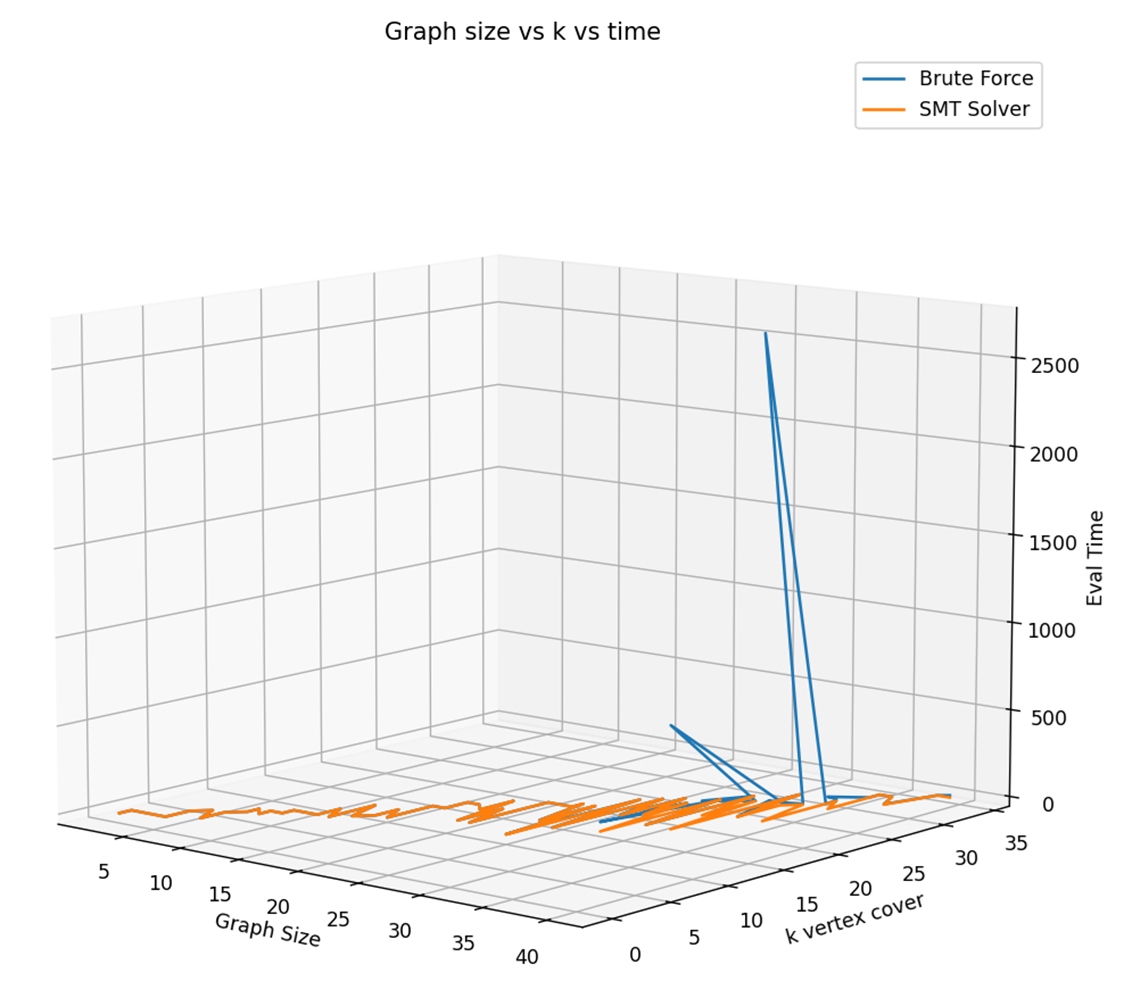
\includegraphics[width=0.6\textwidth]{time_eval.png}
    \caption{Porównanie działania algorytmów w 3d}
    \label{fig:resultsH}
\end{figure}

\subsection{Wnioski}
Jak widać na wykresie, algorytm brute force jest znacznie wolniejszy od algorytmu z wykorzystaniem smt-solvera.
Natomiast rozpatrując każdy algorytm z osobna można zauważyć, że dla brute force rozmiar grafów nie masz aż tak dużego znaczenia, 
tym co wpływa na jego wydajność jest rozmiar szukanego vertex cover. 
Z kolei dla smt-solvera większe znaczenie ma rozmiar grafu niż szukany vertex cover, jednak nie wpływa to znacząco na jego czas działania.
Na podstawie tych obserwacji można wywnioskować, że algorytm z wykorzystaniem smt-solvera jest lepszym rozwiązaniem dla tego problemu.
Należy też brać lekką poprawkę na ograniczenia urządzenia i fakt, że podczas obliczeń mogły wystąpić pewne błędy spowodowane czynnikami zewnętrznymi.

\section{Część I}
\subsection{Opis rozwiązania}
W celu rozwiazania tego zadania, dla każdego algorytmu z osobna, 
empirycznie generowałem coraz większy graf i mierzyłem czas działania programu,
dopóki nie natrafiłem na wynik większy od 2 minut. Starałem się również sprawdzać, 
aby generowany graf miał stosunkowo duży przybliżony rozmiar vertex cover, żeby 
był to bardziej realny przypadek i móc dokładniej określić najlepsze wyniki. 
Przy doborze rozmiaru sugerowałem się także wynikami z części H.

\subsection{Wyniki}
\begin{table}[h!]
    \centering
    \begin{tabular}{cccc}
        \toprule
        Algorytm & Rozmiar Grafu & Vertex Cover & Czas działania (sek.) \\
        \midrule
        Brute force & 30 & 17 & 130 \\
        SMT-solver & 2400 & 2392 & 129 \\
        \bottomrule
    \end{tabular}
    \caption{Tabela przybliżonych wyników dla części I}
    \label{tab:resultsI}
\end{table}

\subsection{Wnioski}
W trakie mierzenia brute force pojawiły się pewne problemy z realnym wynikiem ze względu na fakt, że trzeba zasymulować dokładnie najgorszy przypadek, sugeruje to, 
że czas działania nie jest dużo zależny od liczby wierzchołków lub rozmiaru vertex cover, a bardziej od samego rozkładu grafu i poprawnych w nim wierzchołków.
Zatem można stwierdzić, że brute force mógłby szybko sobie poradzić z bardzo dużym grafem, ale zależałoby to od jego struktury i ustawienia wierzchołków z vertex cover.
Natomiast widać, że smt-solver jest bardziej stabilny i niezależny od tego, jak zbudowany jest graf, co sugeruje, że jest to lepsze rozwiązanie dla tego problemu.
\end{document}